\chapter{Methodology}
\label{chap:Methodology}
\section{Entities}
Throughout this research, four~main entities will be used. These concepts are \begin{inparaenum}[\itshape (i)\upshape]
\item the flight ticket,
\item the airfare~lock-in product,
\item the external company which sells the airfare~lock-in products, and
\item the passenger.
\end{inparaenum}

\subsection{Flight ticket}
A flight ticket gives its holder the right to fly on a particular date and time from and to a particular airport using a specified airline. Flights can be distinct by their unique \emph{call-sign}, which consists of three~different components: \begin{inparaenum}[\itshape (i)\upshape]
\item the IATA airline code,
\item the IATA flight number, and
\item the date of departure.
\end{inparaenum} However, a quick analysis of the data shows that some flights use the same call sign for every leg in a multi-legged route. In this research I have therefore added the departure airport to this sign to make it possible to distinct the underlying legs.

A ticket for a particular flight can be bought many weeks prior to departure. At a certain time, tickets are either available or \emph{sold-out} --- in which an alternate flight with compensation is necessary. In the aviation industry, `\emph{sold-out}' does not always mean that there are no tickets available at a future moment in time. As a result of revenue management and discount allocation, airliners are known to open and close certain \emph{discount buckets} \cite{mcgill1999revenue}. The opening and closing of these buckets prevents missed revenues of high-grossing customers due to actual sell-outs. It is therefore possible that a flight seems to be sold-out weeks before departure, but reappears again closer to the deadline.

The revenue management concept of discount buckets has lead to different prices throughout the booking period. Customers that want to buy a seat for a certain flight earlier to the departure date are likely to be offered other fares than early bookers . Flight tickets are thus dynamically priced.

\subsection{Airfare lock-in product}
The airfare~lock-in products gives its holder the right --- but not the obligation --- to buy the underlying flight on or before a certain maturity date for a predetermined strike price. The holder is thereby covered from sudden increases in price or potential sell-outs, but is still able to not fly at all or gain from large price decreases.

\subsection{External company}
An external company is the entity that offers the airfare~lock-in products to passengers. The seller sets its minimal option prices based upon the expected loss due to increase or sell-out of the underlying flight. The company therefore only accepts to sell the product when the customer will offer a price that is equal or higher than this expected costs.

When the company writes an option, it is thereby obliged to offer the underlying ticket at the specified strike price if the holder exercises it. Flight tickets are capacity constrained, and therefore not unlimited. This means that sometimes the situation emerges in which the option holder wants to exercise its right, but the flight is sold-out. The option writer than has to offer the customer a ticket for an alternative flight plus an extra compensation. The level of compensation could be calculated according to European~Legislation\footnote{\url{http://europa.eu/youreurope/citizens/travel/passenger-rights/air/}}. A sell-out thus creates much increased costs. Therefore, the option price will dramatically increase when the probability of a sell-out is high. In such situations the selling company might refrain itself from offer the option for that particular flight in full.

\subsection{Passenger}
\label{sec:Passenger}
The most central entity in the simulation is the \emph{passenger}.  In this research, a passenger is defined as a customer who considers to purchase a ticket or option for a particular flight on a particular number of days before actual departure of this flight. The distribution of the arrival process for the simulation of passengers will be derived from the article by \citeA{weatherford1993modeling}. In their paper, the authors simulate the arrival according to a inhomogeneous Poisson process. \citeA{bertsimas2005simulation} defined a model more specific for the aviation industry based on the PARM-model.

The simulation model upon which this research is based will only consider the arrival of economy class passengers. This is because the data provide no reliable method of distinguishing different classes, and persons that travel in economy are more price elastic than their business class counterparts. They are therefore more likely to consider an airfare~lock-in product to cover their risk.

\subsubsection{Passenger's decision tree}
When a doubting passenger arrives at the booking process, there is a series of events that might occur. The passenger's decision model is illustrated in \autoref{fig:PassengersDecisionTree}.

\insertfigure{PassengersDecisionTree}{Passenger's decision tree}

First, the customer has to decide whether to \emph{buy the flight} immediately, \emph{wait} a certain amount of time or \emph{buy an option} on the flight and postpone the decision. Next, after a certain period of time, the customer will know whether he will actually take the flight. The probability of flying or not flying is respectively $P^f$ and $1 - P^f$, and is based upon uncertain events that might occur. For instance, the probability of not flying might consist of the probability that the passenger is not able to take a week vacation from work, or even that the weather is bad when the customer wants to go on a sunny holiday.

The action that follows this outcome depends upon the decision made in the first phase. The outcome is calculated by comparing the extra costs incurred by the decision with the `\emph{optimal}' decision that would have been made by a passenger that knew whether he would fly or not ($P^f$ would respectively be $1$ or $0$). The difference of these options is the monetary value of the passenger's \emph{regret} of making his first decision. So, when the passenger decides to actually fly, the costs of his chosen path are compared with the costs of directly buying the flight in the first phase (i.e., $p_I$). On the other hand, when the customer decides not to go, the outcome is calculated by comparing the path with \emph{not buying the ticket in the first place} (i.e., $0$).

\noindent
The different paths that can be followed are
\begin{compactdesc}
\item[buy flight $\rightarrow$ fly] in this scenario, the passenger has already bought the ticket and no further action has to be undertaken. The customer has no regret of making his first decision ($0$);
\item[buy flight $\rightarrow$ don't fly] the passenger will not fly, and the bought ticket is thus rendered useless. The regret of this path is equal to the initial ticket price in the first phase ($p_I$);
\item[wait $\rightarrow$ fly] when the passenger decides to fly after waiting, it will have to buy a ticket. The customer's regret of waiting is equal to the expected price in the second phase minus the initial ticket price ($p_E - p_I$)
\item[wait $\rightarrow$ don't fly] the passenger has to undertake no action, and has not lost any money to a ticket. The customer has therefore no regret of making his first decision ($0$);
\item[buy option $\rightarrow$ fly] the passenger will buy the ticket at the agreed strike price. The extra costs relative to buying the ticket in the primary phase are equal to the option price plus the strike price ($p_S$) minus the initial ticket price. In this research, the strike price will be equal to the initial price, so the customer's regret of making this decision will in this case be the same as the price of the option ($p_O + p_S - p_I = p_O$)
\item[buy option $\rightarrow$ don't fly] the passenger will not exercise the option and will not buy the ticket; The customer's regret is therefore equal to the option price ($p_O$).
\vspace{1ex}
\end{compactdesc}

The expected outcome of each decision made in the first phase can be calculated by multiplying the decision variables $P^f$ and $1 - P^f$ with the result of each branch. The passenger's regret of buying the flight immediately is therefore:
\begin{equation*}
P^f \times 0 + (1 - P^f) \times p_I = (1 - P^f) \times p_I
\end{equation*}

The cost of waiting can be defined as:
\begin{equation*}
P^f \times (p_E - p_I) + (1 - P^f) \times 0 = P^f \times (p_E - p_I)
\end{equation*}

Lastly, the regret of buying an option is:
\begin{equation*}
P^f \times p_O + (1 - P^f) \times p_O = p_O
\end{equation*}

\subsubsection{Passenger's WTP and the third party's WTA}
In a risk neutral setting with equal shared information between option seller and buyer, the price a passenger is willing to pay for the option equals:
\begin{equation}
\min(P^f \times (p_E - p_I), (1 - P^f) \times p_I)
\end{equation}

From the third party's perspective the minimum option price the company is willing to accept is equal to expected incurred costs of selling the product. For a set $\left\{ E(p_1), E(p_2), \ldots, E(p_n)\right\}$ where $E(p_i)$ is the expected result (i.e., $(p_i - p_I) \times P^{\,p_i}$) of price $p_i$ occurring at maturity. The value of $p_O$ can thus be defined as:
\begin{equation}
p_O = \sum\limits_{i=1}^n\begin{cases}
	 E(p_i), & \mbox{if } E(p_i) > 0 \\
	0, & \mbox{if } E(p_i) \le 0 \end{cases}
\end{equation}

This minimum price is related to the costs an option writer expects from selling the airfare~lock-in product. The formula yields the prices at which the company anticipates to lose as much as it gains from selling the option (i.e., the resulting profit from selling this option is $0$).

The equations of the customer's \emph{WTP} and the seller's \emph{WTA} imply that --- in a risk neutral setting --- there will arise an equilibrium between the maximum a customer wants to pay, and the minimum a providing company wants to accepts. This stationary formula for this equilibrium can be defined as:
\begin{equation}
\frac{1}{p_E/p_I} = P^f
\end{equation}

The stationary points are thus dependent on the ratio $\frac{p_E}{p_I}$. This is illustrated by \autoref{fig:StationaryPoints}
\begin{figure*}
	\centering
	\begin{tikzpicture}[domain=1:3]
		\begin{axis}[xlabel=$p_E/p_I$, ylabel=$P^f$]
			\addplot[mark=none] {1/x}; 
		\end{axis}
	\end{tikzpicture}
	\caption{Stationary points}
	\label{fig:StationaryPoints}
\end{figure*}

For combinations of $P^f$ and $\frac{p_E}{p_I}$ that result in an outcome left of the stationary line there is an call option price that both satisfies the passenger and the provider. The combinations to the right of this function do not result in such an option price, and the customer will rather directly buy the flight ticket. An option seller can still target passengers in this area by providing them with a ticket and an option that allows the customers to return the ticket's without additional costs.

\subsubsection{Option style}
\label{sec:OptionStyle}
While customers might be allowed to execute their option during the whole period up till maturity (i.e., American style), I will assume that all options are exercised on the date of maturity (i.e., European option). This is in accordance with the theory of \citeA{merton1973theory}, who states that an American option that does not return dividends should rationally only be exercised at maturity. This assumption can easily be illustrated with the use of an example. If a customer who has bought a real option has decided to exercise the option, it has nothing to lose by waiting till the option matures. By waiting this extra time, the customer only gains an advantage which allows him to still withhold himself from actually buying the ticket. In this way, when there occurs an unforeseen situation after his decision, he still has not bought the ticket and can waive the flight. Therefore it would be unrealistic of the customer to exercise the option before the date of maturity.



\section{Phases}
This research will be divided into three consecutive phases.

The first part, \typenameref{subsec:DataCollectionAndParsing}, will focus on retrieving the pricing-data on a predetermined set of routes. This phase will gather data during a period of 6~weeks and parse it into a new interlinked format. The information retrieved and parsed during this period will be used as the census for the whole study.

The second phase, \typenameref{subsec:OptionValuationModels}, will deal with the analysis of the data and build models around it. To prevent issues like in \citeA{jain11}, the training of the data and testing of the data will be performed on two separate parts: the first 4~weeks of the retrieved data will be used to perform the analysis of the two~different valuation mechanisms, while the lasts 2~weeks is only used to test the models upon. This concept is quite common in machine learning, and prevents the analysis being based on data that is not yet available when the analysis would be performed in real-life.

The third and last phase, \typenameref{subsec:SimulationAndSensitivityAnalysis}, actually tests the previously built models and an optimal one with the use of simulation. This analysis will result in answering the first and third~research question. Next, this phase also consists of sensitivity analysis, which will provide the conclusion for the second~research question.

\subsection{Data Collection and Parsing}
\label{subsec:DataCollectionAndParsing}
In the first phase information on flights will be collected from the Internet. This data will be used as the census for this study. The price setting systems, simulation models and prediction system will all be based upon this dataset.

The website of \href{http://google.nl/flights}{Google Flights} will be used to gather this information. I have selected this resource, because contrary to intermediary sites like Expedia.com, Google Flights does show the lowest available fare and merely redirect users to the airliner's site. Furthermore, direct calls to Google's RPC-server enable users to request XSS-protected JSON-arrays with flight data. See \autoref{app:DataExtractedFromGoogleFlightsRPCRequest} for a detailed list of information included in these arrays.

In this research I will restrict myself to collecting data on 22 different round-trip flights. Of these 22 routes, 10 cover domestic routes within the United~States, 6 are domestic routes within the European Union, and the remaining 6~routes are international. The 10 US domestic flights are two routes selected from the 5 busiest domestic airports within the US, as retrieved from the \citeA{bts13}. The 6 EU domestic flights are a permutation of routes between the airports \emph{AMS}, \emph{CDG} and \emph{LHR}. These three airports are amongst the top~5 busiest airports in Europe \citeA{eur13}. Due to Google Flight's limitation of only providing data for flights departing from the US and the EU, I have selected 6 international routes departing from those areas. See \autoref{app:SelectedRoutes} for the detailed list of selected routes. The routes examined in this study are all round-trip flights with an interval of 7~days between the departure date for the outbound and inbound flight.

\begin{figure*}
\centering
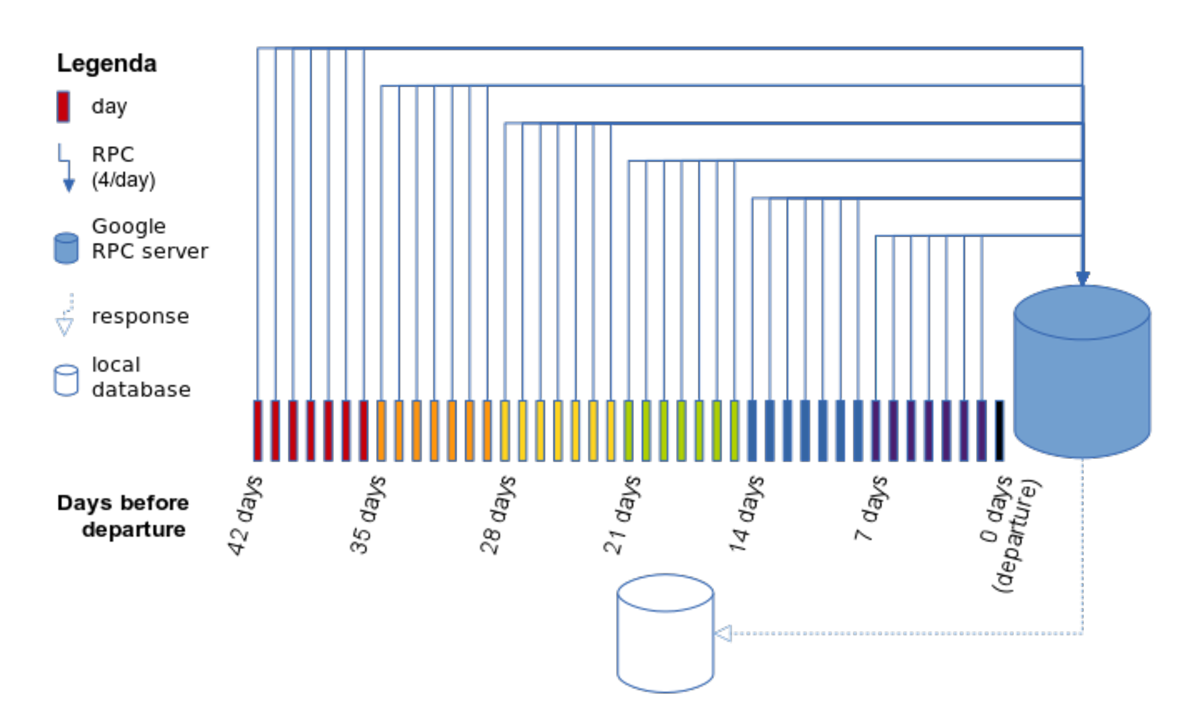
\includegraphics[width=0.8\textwidth]{figures/DataRetrievalProcess}
\caption{Data retrieval process}
\label{fig:DataRetrievalProcess}
\end{figure*}

Data will be collected on the previously mentioned routes departing during the period from Monday the $19^{th}$ of August up until Sunday the $29^{th}$ of September. Price data on all these flights will start 6~weeks prior to departure, up until the day before take-off. The data retrieval can best be illustrated with the help of \autoref{fig:DataRetrievalProcess}. Each day (represented by a rectangular box) an automated program will send a \emph{Remote Procedure Call} (blue arrow) to the \emph{RPC-server} of Google Flights (blue cylinder). This request asks the server to send data on a flight that meets certain specifications. For example, the first call the program makes on July the $8^{th}$ (6~weeks prior to start of collection of specific route) is ``\emph{return data on all flights from ATL to MCO departing on August $19^{th}$ and returning on August $26^{th}$ (7 days after departure)}''. The call is send to the server as a JSON-formatted request (See \autoref{app:SampleJSONRPC} for an example). In return, Google's server will send data on all the flights that meet those requirements (blue dashed arrow) and the automated program will store the received information in a local database (white cylinder). Because Google Flights does not always send back the same flights, the same RPC is send every 6~hours (at 00:00, 06:00, 12:00 and 18:00) \footnote{Each blue arrow thus represents 4 requests on that single day}. The next day the same process is repeated by sending the exact same query to the RPC-server again. This procedure is repeated each day up until the day before departure.

The illustrated process only describes one route (i.e., \emph{ATL} to \emph{MCO}) on one specific date (i.e., departure on \emph{August $19^{th}$}). The automated program however takes into account every route described in \autoref{app:selectedroutes}, and all dates in the period from August $19^{th}$ till September $29^{th}$. The total number of requests made to Google's RPC-server is thereby 22,176 calls \footnote{4 times per day for 7~days per week for 6~weeks for each 22~flights for a period of 6~weeks}.

After retrieval of the flight information, the data is parsed and stored in the \href{http://www.hdfgroup.org/HDF5/}{HDF5-format}. This data format is often used in big data analysis, and enables quick reading of big sets of data to memory. Following the loading into RAM, the data will be converted to a \href{http://pandas.pydata.org/}{Pandas} object after which analysis can be done.

Distinction between flights is made by hashing flight's  properties\footnote{The \emph{call sign} of each segment and \emph{ticketing code} of the flight}. Prices of the flight will be stored in the HDF5-file using the hash as the identification key. This enables easy extraction of price fluctuations within exact same flights relative to time.

\subsection{Option valuation models}
\label{subsec:OptionValuationModels}

% Mun 2006 [jain]: daily return calculation

In this phase the models for option valuation will be built. Currently airliners that offer options on their flights, offer these at a fixed price. This price only differentiates on maturity date, and is equal for all flights and time of purchase. For instance, customers are presented the same price when purchasing the option 1~day or 4~weeks before departure. See \autoref{tbl:PriceOfAirfareLockIn} for examples of current prices at which aviation companies offer fare lock-in products.

\begin{table}[ht]
	\centering
	\begin{tabular}{l  c  c  c  c}
	\hline \hline
	Airline         & 2~days & 3~days  & 7~days  & 14~days \\ \hline
	United Airways  &        & \$\,5.99 & \$\,8.99 & 	       \\
	Air France-KLM  &        &         &         & \$\,20   \\
	Estonian Air    & \$\,15   &         &         &         \\
	\hline
	\end{tabular}
	\caption{Price of airfare lock-in}
	\label{tbl:PriceOfAirfareLockIn}
\end{table}

In this research I will compare three different types of option pricing methods, name\-ly \begin{inparaenum}[\itshape (i)\upshape]
\item an optimal model based upon foreknowledge,
\item a theory-based approach based upon the Black--Scholes model, and
\item a numerical approximation approach based upon the Monte~Carlo method.
\end{inparaenum} The first model is is the theoretical optimal method, while the latter are practically feasible.

\subsubsection{Theoretically optimal: foreknowledge}
The first option valuation model built in this research is based upon the assumption that the option seller knows the exact price of the underlying flight in the future. While this is infeasible in practice, this theoretical model will provide the answer to the first~research question. By using this technique one can conclude whether the external company is able to provide options at a price which the passenger accepts. If it is viable to offer such option in this theoretical setting, more realistic models can be built to see whether it is also feasible in the practical world. Furthermore, this optimal method will be used as baseline to compare the other two models. 

\subsubsection{Theory-based: Black--Scholes model}
The Black--Scholes model will be the first practical implementations of a option valuation technique in this research. The model is used to determine the European option price based upon the volatility of the underlying asset. \citeA{jain11} demonstrated in their paper that this model can also be used to determine optimal option prices based on the volatility of airfares. In this paper, I calculate the volatility of the airfares by using the first 4~weeks of the census. With this variable, the optimal option price according to the Black--Scholes method can be calculated, and the outcome can be tested in the simulation model. The adapted equation used for this flight specific scenario is derived from \citeA[p.~13]{jain11}:
\begin{align*}
p_O &= p_I \times N(d_1) - p_S \times e^{-rT}N(d_2) \\
d_1 &= \frac{\ln(p_I/E) + (r + \sigma^2/2)T}{\sigma \sqrt{T}} \\
d_2 &= d_1 - \sigma \sqrt{T}
\end{align*}
See \cref{app:AdaptedBlackScholesFormula} for a full description of the equation.

\subsubsection{Numerical approximation: Monte Carlo}
The next practical implementation of an option valuation technique is the Monte~Carlo method. This model is more flexible and can be used when the underlying returns do not follow a log-normal distribution. Furthermore, as \citeA{walker1998method} states, options on flights are quite different from options found in the financial market. The main differences are \emph{non-interchangeability} and \emph{capacity restrictions}. A Monte~Carlo can be configured in such a way that it also takes into account such distinctions.

\citeA{richardson2009numerical} gives an example implementation of the Monte~Carlo method to set the prices of options. Instead of volatility and random returns, I will implement this model based upon the expected returns seen in the training~set of the data. The outcomes will be tested using the designated set of the data, and relatively compared with the optimal model.


\subsection{Simulation and sensitivity analysis}
\label{subsec:SimulationAndSensitivityAnalysis}
In the third phase the three pricing models described in \typenameref{subsec:OptionValuationModels} will be evaluated using simulation.

This simulation model generates passengers that want to buy tickets of a certain flight as a function of time (6~weeks till one day before departure). 

To make sure the models are not overfitted on the train data, the simulation will be run on the separate set of test data.

\subsubsection{Sensitivity Analysis}
During the simulation a sensitivity analysis will be performed as well. In this analysis the three~parameters of a passenger --- \begin{inparaenum}[\itshape (i)\upshape]
\item risk-utility,
\item forecasting technique, and
\item likelihood of travelling.
\end{inparaenum} --- will be altered to see what the effect of these properties is on the price setting model.
